\documentclass[english,11pt]{article}
\usepackage{url}
\usepackage{threeparttable}
\usepackage{geometry}
\usepackage{lscape}
\usepackage{tabularx}
%\usepackage{mdwlis}

%%%%%%%%%%%%%%%% Reasonable Margins
\setlength{\textwidth}{6.5in} \setlength{\textheight}{9in} % 6.2 and 8.5 normal...
\setlength{\topmargin}{-1.1in} \setlength{\oddsidemargin}{0in}
\setlength{\parskip}{2mm}
\usepackage{paralist}
\usepackage{amsmath}
\usepackage{amssymb,epsfig,amsthm,amsfonts,bm}
\usepackage{graphicx}
%\usepackage[T1]{fontenc}
%\usepackage[ansinew]{inputenc}
%\usepackage{a4}
\usepackage{babel}
\usepackage{array}
%\usepackage{natbib}
\usepackage{cite}
%\usepackage{biblatex}
\usepackage{xr}
\usepackage{setspace}
\usepackage[small,bf]{caption}%[1995/04/05]
\usepackage[dvipsnames]{xcolor}
\usepackage{color}
\usepackage{dcolumn}
\usepackage{lscape}

\newcolumntype{.}{D{.}{.}{1}}
%\setlength{\abovecaptionskip}{-0.01cm}
%\setlength{\belowcaptionskip}{0.05cm}
%\usepackage[ruled,vlined]{algorithm2e}
%\usepackage{algorithm, algpseudocode}%loads algorithmicx
%\usepackage{algorithmicx}
\everydisplay{
\abovedisplayskip=.47\baselineskip  plus.2ex minus.2ex
\abovedisplayshortskip=-0.13\baselineskip plus.2ex minus.2ex
\belowdisplayskip=.37\baselineskip plus.2ex minus.2ex
\belowdisplayshortskip=.37\baselineskip plus.2ex minus.2ex
}

% nothing command
\newcommand{\nothing}[1]{}
\usepackage{arydshln}
\usepackage{booktabs}
\usepackage{array,hhline}
\usepackage{rotating}
\usepackage{tabularx}

\newcommand{\blue}[1]{{\color{RoyalBlue}#1}}

\usepackage{soul}
\setlength{\parskip}{1.5ex plus 0.5ex minus 0.5ex}

%\DeclareMathOperator{\Cov}{cov}
\newcommand{\E}{\mathbb{E}}    % E, expectation
\newcommand{\Var}{\mathsf{Var}}% Var, variance
\newcommand{\Cov}{\mathsf{Cov}}% Cov, covariance
\newcommand{\EWMA}{\mathsf{ewma}}% Cov, covariance
\usepackage{paralist}

% font
\usepackage[T1]{fontenc}
%\usepackage{lxfonts}


\definecolor{DarkBlue}{rgb}{0,0.0,0.5}
\definecolor{DarkGreen}{rgb}{0.01,0.4,0.01}

% THEOREMS
\newtheorem{theorem}{Theorem}[section]
\renewcommand\qedsymbol{$\blacksquare$}
\newtheorem{cor}{Corollary}
\newtheorem{lemma}{Lemma}
\newtheorem{proposition}{Proposition}
\newtheorem{defn}{Definition}
\newtheorem{rem}{Remark}
\newtheorem{assumption}{Assumption}
\newtheorem{hypo}{Hypothesis}

% <thanks symbol>
\makeatletter
\renewcommand*{\@fnsymbol}[1]{\ensuremath{\ifcase#1\or *\or **\or ***\or
   \mathsection\or \mathparagraph\or \|\or **\or \dagger\dagger
   \or \ddagger\ddagger \else\@ctrerr\fi}}
\makeatother
% </thanks symbol>

% short comment
\def\query#1{\marginpar{\begin{flushleft}\textcolor{red}{\footnotesize#1}\end{flushleft}}}%
% longer comment
\def\cmnt#1{ \textcolor{red}{#1} }
%\onehalfspacing
% rephrasing
\def\rephr#1{\textcolor{blue}{#1}}

%\onehalfspacing


\title{Frankencoin\thanks{Preliminary}}
\bigskip
\bigskip



{
\date{ \today  }


\author{
Luzius Meisser\thanks{\texttt{luzius.meisser@gmail.com}}\\
\emph{Meisser Economics}
\and
Basile Maire\thanks{\texttt{basile.maire@desma8.io}.} \\
\bigskip
\emph{Desma Eight, LLC}

}

\bigskip
\bigskip

\bigskip
\date{\today }




\newpage
\newpage
\begin{document}

%\nothing%blind

%%%%%%%%%%%%%%%%%%%%%%%%%%%%%%%%%%%%%%%%%%%%%%%%%%%%%%%%%%%%%%%%%%%%%%%%%%%%%%%%%%%%%%%%%%%%%

	\newpage
	\thispagestyle{empty}
	
	\vspace{2.5cm}
	
	\thispagestyle{empty}
	
	\vspace{2.5cm}
	\smallskip
	\centerline{\bf {\Large Frankencoin }}
	
	\vspace{.5cm}
	\begin{abstract}
	blabla
	\end{abstract}
	\bigskip
	\bigskip
	
	%vspace{1cm}
	\noindent{\it JEL Classification Codes: D40, G23}
	
	%\vspace{1cm}
	\bigskip
	%{{\noindent \it{Key Words}: 
	%}  }
	
	
	\bigskip

	\newpage
%>>>\tableofcontents

	\newpage

\setcounter{page}{1}

% !TEX root = ./perpetual.tex
%%%%%%%%%%%%%%%%%%%%%%%%%%%%%%%%%%%%%%%%%%%%%%%%%%%%%%%%%%%%%%%
\section{Introduction}
We start from the use-case of a Swiss Frank Lombard loan, collateralized with tokens such as Bitcoin, or tokenized shares. The borrower deposits collateral into the system and thereby
mints a token, the ``Frankencoin'' ZCHF, that is pegged to the Swiss Frank. If the value of the borrower's collateral falls below a certain threshold, the loan can be liquidated and the borrower incurs a haircut. If the value of the collateral falls below the loan value before the liquidation ends, the loss eats into capital. Implementing this system in
a fully decentralized way on the Blockchain leads us to our main contribution.

First, we introduce an algorithmic stablecoin that allows for 
\emph{different collateral types and liquidation rules}.
This diversification of collateral and liquidation rules reduces the 
impact of non-systemic market events to the stablecoin peg.
Second, we propose a specific mint plugin setup for which
\begin{itemize}
\item We use an \emph{auction mechanism} that avoids using external Oracle price feeds
\item To calibrate the system, we apply traditional risk management techniques that have not found their way into the world of stablecoins
\end{itemize}

The system entails a decentralized governance that governs risk parameters and can deny the community's addition of new peg-methodologies if deemed unfit.

The Frankencoin can be minted by anyone using one of the available 
mint plugins. We define mint plugins as smart contracts that have the ability to mint Frankencoin in accordance with their rules. 
Mint plugins have to be approved by the governance msimilarechanism and there might be different types of mint plugins for different types of collateral and different liquidation mechanisms. Anyone can propose to add a new mint plugin and if it is approved by the governance mechanism, it can be used according to its rules. These rules can include interest rates that are owed by the minters, liquidation mechanisms, collateral requirements, and required ZCHF
to be held by ``stakers'' as a reserve per ZCHF token minted.
While every mint plugin defines their required reserve capital,
the reserves are shared among all mint plugins.

Stakers are participants that lock their Frankencoin into the system. 
Stakers
earn interest rates paid for by borrowers and in turn risk
to lose Frankencoin in case the liquidation process is not able to recover
the loan amount with the available collateral.
Staked Frankencoin are subject to a lockup period. This ensures that in case of a "bank run" on the system, stakers are the last who can liquidate their Frankencoin and will therefore also suffer from the greatest losses while the other participants are likely to be able to reclaim the full value.

This paper focuses on two aspects of Frankencoin. First, we discuss
how the Frankencoin embeds with the wider economy. Many
existing stablecoin systems fall short of this aspect and can
arguably only be sustained with significant growth of the system
or demand of their own token, see e.g., \cite{clements2021built}.
We propose a specific setup of mint plugins for which
we use standard risk methodology techniques
to quantify adverse events and calibrate
capital reserves and fees. This is in stark opposition
to existing stablecoins that set parameters such as the
collateralization-ratio without risk methodological quantification
methods. \emph{TODO: reference??}

\section{Economy}
The immediate participants of Frankencoin consist of 
\emph{minters}, \emph{users}, and \emph{stakers}.

\emph{Minters} deposit collateral into a mint plugin and thereby
enter a Frankencoin Lombard loan. Minters benefit from the system to the extent that it allows them to use liquid or illiquid assets that
they want to hold long-term, to generate short-term liquidity. This
can be motivated e.g., by tax considerations in some juristicions, or
by justifications that hold for traditional Lombard loans.
Similar to Lombard loans, the position is overcollateralized.

\emph{Stakers} stake Frankencoin in a dedicated contract, thereby locking
these funds up for a certain period of time. As a consequence, stakers 
are the last to be able to liquidate their holdings in case of a collapse of the value of Frankencoin. Stakers have to be compensated for their risk. 
This compensation is provided by the minters. Fees and interest rates
paid by the minters are distributed to the stakers. By staking Frankencoin,
stakers release governance tokens that give them voting rights.

\emph{Users} hold and transfer Frankencoin as a means of payment or
store of value. No fees are charged to the users, but they also are not provided with any financial gain from holding Frankencoin by the system. The system should be designed such that the tail risk of a complete default is negligible for the users as that risk is outsourced to the stakers.

This setup separates risk-takers (stakers) from the users.
Governance token holders have "skin in the game" and are thus
incentivized to maintain a healthy system.
For instance, because staker capital is shared for all mint plugins, 
stakers have a vested interest to retain a healthy ecosystem of mint plugins.

Creditors of Frankencoin loans should be paid a risk-free rate
corresponding to the Swiss Frank, plus a risk-premium. Otherwise,
there is no rationale why stakers should sustainably 
lock their funds in Frankencoin (other than for non-pecuniary reasons).
From the perspective of the minters, this means that costs to minters 
should be in line with the market capital costs for their loan.

We now address the conditions
under which the \emph{peg to the Swiss Frank} should hold.
We approach the valuation of the Frankencoin from the perspective
of a \emph{perpetual bond}. A perpetual bond, or consol, is
a bond with coupon payments but no redemption date, see, e.g.,
\cite{jorion2010financial}.
The staked Frankencoin is subject to default risk, because the system
burns ZCHF when a minter's position is undercollateralized. 
We price this credit-risky perpetual along the lines of \cite{jarrow2000derivative},
by discounting the interest payments on a credit-risky term structure.
Let's assume that interest payments happen at discrete time-steps $0,...,\infty$
and we have corresponding risky rates of the term-structure
so that the date-0 value of a promised Swiss Franc at time $t$ of a credit-risky
Franc promise is equal
to $\exp(-r_t t)$. Let the constant coupon rate per Frankencoin be $c$. 
Now, the value of the perpetual can be written as
\begin{align}
v(0) &= \sum_{t=0}^{\infty} c e^{-r_t t} \\
	 &= \sum_{t=0}^{\infty} c e^{-y t} \\
	 &= \frac{c}{1-e^{-y}},
\end{align}
where the second line replaces the time-specific discount rates by
a yield, and the last line is an application of geometric series.
For the value to be at par, $v(0)=1$, we have to choose the coupon rate
accordingly: $c = 1-e^{-y}$. Hence, if the interest earned from staking 
ZCHF are in line with discounting, the present value of one ZCHF is equal 
to one Swiss Franc.

The credit risky term-structure corresponds to the Swiss Franc risk-free term-structure
plus a spread that compensates the investor for the risks. 
Hence whenever the risk-free term-structure, or the Swiss Franc risk
changes, $c$ hast to be adapted for the value $v(0$) to be equal to one.
This is difficult to automate, and
we therefore allow the stakers to collectively set the interest 
rate (i.e., the risk-free rate plus spread). That is, if the 
exchange rate of the ZCHF is too low, the stakers use the governance mechanism to increase the interest rate and vice versa.

We design the system so that it is in the interest of the stakers 
to set the parameters of the system such that the peg is maintained. 
There should be no abuse of power, for example to set interest rates too high, therefore pushing the value of their ZCHF way beyond one CHF and essentially stealing the collateral as it would become too expensive for the minters to buy ZCHF to get their collateral back. To prevent such an attack, we ensure that stakers can only slowly adjust the interest rate, 
so that it is possible for the participants to trade-in their ZCHF 
before rates are too punitive (e.g., minters redeem their collateral by repaying their loan).

The next section presents a specific setup of mint plugins and proposes
a calibration method to determine the appropriate spread that should
bring the value of the Frankencoin close to a valuation of one Swiss Franc. 

\section{Specific Mint Plugin Setup}
The Frankencoin system is open to accept any type of mint plugins. 
In this paper we describe a setup with two specific mint plugins that 
we consider to be of particular relevance when bootstrapping and growing the Frankencoin.

Each mint plugin $i \in 1,...,K$ charges a minting fee $\Theta_{i}^{(F)} \geq 0$, and can define
a coupon rate paid to stakers $\Theta_i^{(I)} \geq 0$. Depending on the plugin type,
there can be additional plugin-specific parameters.

\subsection{Direct Peg Plugin}
The simplest possible mint plugin is one that is based on a stablecoin with the same reference currency. Specifically, "off-chain" custodial stablecoins. For the Frankencoin, this could for example be the CryptoFranc (XCHF) issued by Bitcoin Suisse or the Digital Swiss Franc (DCHF) issued by Sygnum. 
This mint plugin allows anyone to deposit the specified stablecoin and to get Frankencoins in return. Also, the minting contract would allow anyone to convert Frankencoins back into the specific stablecoin for as long as there are any left.

Direct peg plugins have the advantage of strongly anchoring the value of the Frankencoin to one Swiss Franc by delegating the collateralization mechanism
(e.g., directly backed by Swiss Francs).  
The disadvantage for direct peg plugins is the dependency on 
the issuers. Overall, direct peg are a great method to bootstrap 
the Frankencoin and diversify the Frankencoin system.

\subsubsection{Fee Calibration}
In case of issuer default, stakers have to burn ZCHF equal to the amount of
loss given issuer default times the exposure to that stablecoin. 
To compensate stakers for this risk,
we charge a minting fee. Again, we have the advantage that 
calibration is outsourced to the market.
If the value of one stablecoin trades at $1-\delta$ to the Swiss Franc, governance
sets a minting fee equal to $\Theta_F^{(i)} = \delta$.

\subsubsection{Reserves}
Each mint plugin defines the required reserves of ZCHF to be held against
the issued volume of ZCHF. XCHF and DCHF come with their own guarantee
that extend beyond the issuer default. Therefore, for the direct peg 
plugin and XCHF and DCHF as collateral, we require no reserves.

\nothing{
To guard against default risk of an issuer, minting should be limited to the staked amount of Frankencoins in the governance contract. That way, the Frankencoin could absorb a total loss of value of one of the pegged stablecoins. In case of a loss of trust in the pegged stablecoin, it would be challenged in a vote of distrust the remaining coins auctioned off, with the stakers having to take a loss in case the auction does reach a 1:1 conversion rate.
}

\subsection{Liquid Collateral Plugin}
The second type of mint plugin is designed for liquid collateral, such as
Bitcoin. This type of plugin implements the use case of a Lombard loan that
we motivated the paper with.

\begin{itemize}
\item The participants are minters, challengers, auction participants, and ZCHF stakers.
\item The minter deposits collateral and thereby mints ZCHF. The ZCHF are overcollateralized at the time
of minting, that is, the value of collateral deposited exceeds the value of the minted ZCHF.
\item Challengers can initiate an auction process for a given position at any time.
To do so, they deposit collateral of the same type. 
After the challenge initiation, auction participant bid for the collateral by despositing
ZCHF.
\begin{enumerate}
\item If, according to the auction, the value of the collateral falls below a specified threshold, the position is liquidated
and the minter loses their collateral. \emph{E.g., the collateral deposited is 1500 LUSD, 1000 ZCHF were minted. Now, the position
is challenged and the best bid for 1500 LUSD closes at 1095 ZCHF. Let's assume that the threshold is 10\%. Now, because 
1095 ZCHF < 1000 (1+10\%) ZCHF, the position is closed out.}
The challenger earns a fee, and the bidder gets the the collateral he was bidding for.
The ZCHF posted by the bidder are distributed as follows. The challenger
receives a reward. An amount equal to the outstanding loan is burned:
\begin{itemize}
\item If any ZCHF above the loan amount is left, the stakers get this amount
\item If the posted ZCHF are not sufficient to burn an amount equal to the outstanding loan,
the stakers lose this amount
\end{itemize}
\item If, according to the auction, the collateral value is above the threshold, the position remains in the minter's ownership. The bidder gets the challenger's collateral and
the challenger get's the bidder's amount of ZCHF.
\end{enumerate}
\end{itemize}

Figure~\ref{fig:auction} illustrates this auction mechanism graphically.
\begin{figure}[h]
    \center
    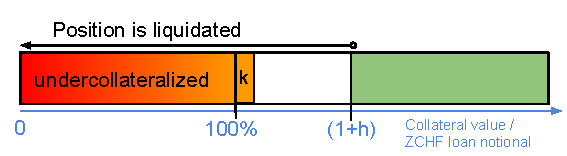
\includegraphics[width=0.75\textwidth]{auction.pdf}
    \caption{\textbf{Auction}. Any participant can challenge a
    loan position consisting of the ZCHF loan and the deposited collateral.
    The challenger deposits collateral of the size of the loan.
    Auction participants bid for the collateral (here BTC) by depositing ZCHF. 
    If the best bid price in ZCHF is above (1+h) times the notional ZCHF lent,
    the challenger receives the best bidder's ZCHF and the bidder the challenger's
    collateral (green zone). If the best bid price is below (1+h),
    the borrower loses their collateral (position is liquidated).
    In this case the challenger gets back their collateral and earns a fee of
    $k$ times the loan amount. The bidder gets the collateral deposited
    by the borrower. The ZCHF posted by the bidder are used to
    pay a reward $k$ to the challenger, $(1+h-k)$ times the loan amount 
    go to the staking pool, and an amount equal to the loan 
    amount is burned. If the ZCHF are not sufficient to burn
    an amount equal to the loan amount after paying $k$, stakers have
    to burn this amount of ZCHF. Hence the unshaded area
    in the center is where stakers earn liquidation rewards,
    the area to the left is costly for stakers.}\label{fig:auction}
\end{figure}

Our liquid collateral mint plugin has the following parameters. Variable $h$ denotes the threshold that defines whether the position
can be liquidated or not. That is, if, according to the auction, the value of the collateral is below 
$Z(1+h)$, where $Z$ is the amount of ZCHF minted for a given position, the position is liquidated.
Variable $k$ denotes the challenger reward (e.g., 2\% of the ZCHF position). 
Finally, $\tau$ is the duration of the auction (e.g., 24 hours). To summarize:
\begin{align}
h &: \text{$h>0$, liquidation threshold, liquidate if highest bid is below Z(1+h)}\\
\tau &: \text{duration of liquidation process}\\
k &: \text{$0<k<h$, challenger reward}
\end{align}

Since our choice of collateral is liquid and can be traded at many different venues,
we expect arbitrageurs to bid in the liquidation process and arbitrage
between the liquid collateral mint plugin and other exchanges.
This is best done via algorithmic trading, and we therefore propose to use a short
liquidation horizon (hours, rather than days).

We define an "efficient liquidation process" as the situation in which
the collateral is challenged at a price $(1+h)$, and at the end of the
liquidation period $\tau$, the collateral is sold at a competitive price.
In practice, likely the challenge will not be issued at a price $(1+h)$ but
rather at a lower price $(1+h')$ where $h'<h$.
We proceed by setting the period $\tau$ to 24 hours and calibrate the remaining parameters:
$h$, $h'$, $\Theta_F^{(i)}$.

\subsubsection{Fee Calibration}
Stakers are at risk to lose funds between the liquidation start and liquidation end.
Specifically, if during the liquidation horizon the value of the collateral drops 
from $(1+h')$ to below $(1+k)$, see Figure~\ref{fig:auction}.
The key challenge now is to value this risk so that the stakers
are adequatly compensated.

We have a single period, of duration $\tau$, a random
variable, $\tilde{r}_{\tau}$, that corresponds to the log-return of the collateral over this period (using CHF as the numeraire).
Now, we can express the loss to the stakers as the following random variable:
\begin{align}
\tilde{L} = - \left[(1 + h') e^{\tilde{r}_{\tau}} - (1+k)\right] \mathbf{1}_{\tilde{r}_{\tau}<\log \frac{1+h}{1+h'}},\label{eq:loss}
\end{align}
per unit of ZCHF minted (e.g., if the position consists of $Z$ ZCHF, the loss to the stakers is $Z\tilde{L}$).
To see this, first note that the starting value of the position is $(1 + h')$ per unit of $ZCHF$.
The value of the position
at the end of the auction is $(1 + h') e^{\tilde{r}_{\tau}}$. Stakers need to burn ZCHF for the amount that the end-of-auction value falls short
of the minted amount plus the challenger reward, hence we subtract $(1+k)$. 
Second, the stakers earn in the liquidation process only if the return $\tilde{r}_{\tau}$ leads to a value below $(1+h)$, otherwise
there is no liquidation, see
Figure~\ref{fig:auction}, so we need the indicator function $\mathbf{1}_{.}$ that equals one if
\begin{align}
\text{condition for liquidation:} \qquad(1+h')e^{\tilde{r}_{\tau}} < (1+h)\label{eq:liqcond}
\end{align}
holds, zero otherwise. Note that if the liquidation starts at $h'=h$, 
the indicator function simplifies to $\mathbf{1}_{\tilde{r}_{\tau}<0}$.
Finally, the negative sign is 
convention to have a positive number for a loss and a negative number for gains.

To tackle the valuation of $\tilde{L}$, we resort to the arbitrage free pricing principle,
which states that the value of a contingent claim is given by
its discounted expected value under the risk-neutral probability measure,
see for example \cite{bjork2009arbitrage}.
We assume that the risk-free rate used for discounting is equal to zero,
which we consider adequate especially since the period $\tau$ is very short.
Let $f_{\tau}(x)$ be the density function for the return distribution over the period $\tau$. Now, we can value $\tilde{L}$ conditional
on the starting level of liquidation $h'$ as follows
\begin{align}
\mathbb{E}_{\tau}\left[\tilde{L} \vert h' \right]  &= - \int_{-\infty}^{\log \frac{1+h}{1+h'}} \left[(1 + h') e^{x} - (1+k) \right] f_{\tau}(x) dx\label{eq:E}
\end{align}
where the subscript $\tau$ emphasizes that the distribution depends on the time-horizon of the auction.
If we knew the distribution of starting levels $h'$, we could integrate out $h'$ to arrive at $\mathbb{E}_{\tau}[\tilde{L}]$.

We now discuss $h'$. The challenger does not receive the challenger reward in case the auction finalizes at a price above $(1+h)$, but 
they instead swap their collateral posted against the best ZCHF bid. Even if the challenger is likely to
get a competitive price, they are arguably more interested in collecting the 2\% liquidation 
reward than performing a trade. From this perspective, the challenger would be better off not starting the challenge
at $(1+h)$ but a price quite below that to increase the probability that the auction ends below $(1+h)$. However,
if the challenger target too low entry points, other challengers could enter above, or prices could correct to above $(1+h)$
so that no more challenge is possible.
Hence, challengers trade off the probability of collecting the reward given they issue a challenge versus the probability of not being able to enter
a challenge anymore. To investigate this trade off, we assume that challengers issue a challenge when the collateral value
reaches a level for which there is a probability $\alpha$ that they receive the challenger reward. Formally, using
Equation~\eqref{eq:liqcond}, we determine
$h'$ so that the following equation holds:
\begin{align}
	%\mathbb{P}[(1+h')e^{\tilde{r}_{\tau}} < (1+h)] = \alpha \\
	\mathbb{P}\left[\tilde{r}_{\tau}<\log \frac{1+h}{1+h'}\right] = \alpha,\label{eq:hdash}
\end{align}
for a given $\alpha$. We then assume that the liquidation level is given and equal to the value $h'$ that solves \eqref{eq:hdash}.

Equation~\eqref{eq:E} uses the risk-neutral probability measure, often referred to as
$\mathbb{Q}$, rather than the objective measure $\mathbb{P}$. In practice,
parameters for the measure $\mathbb{P}$ are extracted directly from market data
(e.g., sample volatilities and expected returns), whereas
parameters for the measure $\mathbb{Q}$ have to be extracted from option data
under the same model assumptions (e.g., option implied volatilities). 
With risk averse investors, the $\mathbb{Q}$-measure puts more
weight on adverse market events, see for example \cite{breeden1978prices}, leading
to a higher risk-neutral price of $\tilde{L}$, compared to the value obtained
when integrating Equation~\eqref{eq:E} under the objective measure.
We therefore proceed by calibrating a probability distribution to observed
market data and use this as a lower bound for the price of $\tilde{L}$, or,
equivalently the minting fee should be at least equal to the price of $\tilde{L}$:
\begin{align}
\Theta_F^{(i)} \geq \mathbb{E}_{\tau}\left[\tilde{L} \right].
\end{align}

We are now ready to calibrate the parameters. To do so, we set the level $\alpha$ 
to estimate $h'$, and then estimate the fee $\Theta_F^{(i)}$ for the given level of $\alpha$.
In Appendix~\ref{appx:data} we describe the BTCCHF data that we use to calibrate the
fees. The normal distribution does not fit the empirical distribution of 24-hour log-returns well, as we demonstrate in the appendix.
Therefore, instead of fitting another parametric distribution and integrating Equation~\eqref{eq:E}, we use 
the bootstrap method introduced by \cite{efron1992bootstrap} for estimation.

For the bootstrap, we define the following variables. Let $N$ be the number of return observations, $B$ the number of bootstrap replications,
and let $\mathbf{\hat{r}}_b = \{\hat{r}_{\tau}^{(b,1)},...,\hat{r}_{\tau}^{(b,N)}\}$ be
the $b^{th}$ bootstrap replication. We use the variance of the quantiles for each bootstrap replication to estimate confidence intervals.

We can estimate $h'$ for a given $\alpha$ using Equation~\eqref{eq:hdash}, by extracting the sample quantile from
each bootstrap replication:
\begin{align}
	\hat{h}' = \frac{1}{B} \sum_{b=0}^{B-1} Q((1+h)\exp(-\mathbf{\hat{r}}_b)-1, 1-\alpha),
\end{align}
where $Q(\mathbf{x}, a)$ is the empirical quantile function for level $a$ applied to vector $\mathbf{x}$, 
and we define $\exp(\cdot)$ to be an element-wise application of the natural exponentiation.
Finally, we use use Equation~\eqref{eq:loss} 
to arrive at our bootstrap point estimate for the value of $L$:
\begin{align}
\mathbb{\hat{E}}_{\tau}\left[\tilde{L} | h' \right] &= - \frac{1}{BN} \sum_{j=0}^{B-1} \sum_{n=1}^N 
	\mathbf{1}_{\{\hat{r}_{\tau}^{(jN+n)}<\log \frac{1+h}{1+h'}\}} 
	\left[(1 + h') e^{\hat{r}_{\tau}^{(j,n)}} - (1+k)\right].
\end{align}
Again, we use the variance of the elements from each bootstrap replication to estimate confidence intervals.

Table~\eqref{tab:calibration} shows the results of the calibration. We use $B=5,000$
bootstrap replications and calculate confidence intervals at the 1\%-level by applying
the central limit theorem, that is, recycling the variances described above and 
normal-quantiles.\footnote{Having a vector of bootstrap estimates 
$\mathbf{x}$, we report the point estimate as the mean of $\mathbf{x}$, and the
error at the a-level as $z_{1-a}\sqrt{V[\mathbf{x}]/B}$ with $z_{1-a}$ the standard normal quantile.}
In Table~\eqref{tab:calibration}, we see that if the challenger want a 95\% chance of earning
the challenger reward, they start the challenge at $(1+3\%)$. At this low level, the 
stakers still make a profit of 0.63\% on average. From the first row of the table, we 
see that if the challenger starts their challenge at the liquidation level of $(1+0.1)$,
there is about a 50\% chance that the position will be liquidated at the end of the
24h-period. The earnings for the stakers decrease when moving from $h'=0.10$ to a
lower $\alpha$. This is because in many cases, the stakers have no profit when
starting from $0.10$, because there is no liquidation, and hence, the expected profit
is slightly higher when starting from a lower $h'$.
From the last row of the table we see that if challenges are issued only after the
collateral fell below the loan value by 1\%, the stakers expect a loss of 2\%.

A 95\% probability of receiving a challenger reward seems a very good position
to be in for the following reason. The challenger at this point has the option of 
waiting for the prices to change more.
The collateral could either depreciate more (which would increase
the 95\% chance of getting the reward), or appreciate, in which case the probability
is decreased. So very likely at this point, the challenger would issue the challenge.
At $\alpha=0.95$, the stakers still earn on average. Therefore we conclude
that for the Liquid Collateral Plugin collateralized with Bitcoin and the chosen risk parameters,
no minting fee has to be charged, unless the risk-premium exceeds about 0.60\%.

\begin{table}[h]
\caption{\textbf{Liquid Collateral Minting Fees.} The column labelled $\alpha$ shows the probability
that the challenge results in a liquidation and the challenger is paid a reward.
The second column shows the challenge level $h'$ for which the challenge ends in a
liquidation with probability $\alpha$ for a liquidation level $h=10\%$ and a challenge
period of 24 hours. For each given $h'$ we calculate the expected loss for the stakers
(last column; negative numbers are gains).
The numbers followed after $\pm$ correspond to the error of our estimates at the 1\%-level.
We see that if challenges are issued at a collateral value of $(1+0.03)$, quite below the 
liquidation level of 1.1, there is
a 95\% probability that the collateral is liquidated, while stakers will still on average
earn 0.69\%.\label{tab:calibration}}
\center
\begin{tabular}{lll}
\toprule
\textbf{$\alpha$} & \textbf{$h'$}   & \textbf{$\hat{E}_{\tau}\left[\tilde{L} | h' \right]$}\\
\midrule
0.50                           & 0.10 $\pm$ 0.00 & -2.59\% $\pm$ 0.00\% \\
0.75                           & 0.08 $\pm$0.00  & -3.30\% $\pm$ 0.00\% \\
0.80                           & 0.07 $\pm$0.00  & -3.21\% $\pm$ 0.00\% \\
0.90                           & 0.05 $\pm$0.00  & -2.37\% $\pm$ 0.00\% \\
0.95                           & 0.03 $\pm$0.00  & -0.63\% $\pm$ 0.00\% \\
0.99                           & -0.01 $\pm$0.00 & 2.99\% $\pm$ 0.00\% \\
\bottomrule
\end{tabular}
\end{table}

\clearpage
\subsubsection{Reserves}
Each mint plugin defines the required reserves of ZCHF to be held against
the issued volume of ZCHF. In the previous section we have calibrated
the minimal fee that should be charged to minters via expected loss.
We proceed in a similar manner and calculate the expected shortfall
for the liquidity providers under a 1\%-quantile, conditional on $h'$.

We bootstrap the expected loss:
\begin{align}
EL_{\gamma} &= - \frac{1}{B} \sum_{b=0}^{B-1} \frac{1}{|\{ \hat{r}_{\tau}^{(b,n)} < Q(\mathbf{\hat{r}}_b, \gamma) | n=1,...,N \}|} \sum_{n=1}^N 
	\mathbf{1}_{\{ \hat{r}_{\tau}^{(b,n)} < Q(\mathbf{\hat{r}}_b, \gamma) \}} 
	\left[(1 + h') e^{\hat{r}_{\tau}^{(b,n)}} - (1+k)\right].
\end{align}
Table~\ref{tab:calibration2} shows the results. We can see that with a conservative assumption of 
challengers entering when the probability of earning the reward is $alpha=90%$, stakers
face a 15\% average loss in the worst 1\% outcomes. We choose this number, 15\%, as our conservative risk-based
buffer $\Theta_i^{R}$.

\begin{table}[h]
\caption{\textbf{Liquid Collateral Capital Reserves.} The column labelled $\alpha$ shows the probability
that the challenge results in a liquidation and the challenger is paid a reward.
Given this level, we can calculate the corresponding $h'$, see Table~\ref{tab:calibration}.
The last second column shows the expected shortfall at the 1\%-quantile. The value
after $\pm$ is the confidence area at a 1\%-limit. For example, if challengers wait to issue a challenge until
there is a 90\% chance that they receive a challenger reward, the average loss in the worst 1\% of outcomes
is equal to 15\%.
\label{tab:calibration2}}
\center
\begin{tabular}{lll}
\toprule
\textbf{$\alpha$} & \textbf{ES}   \\
\midrule
0.50                           & 0.11 $\pm$ 0.00 \\
0.75                           & 0.13 $\pm$ 0.00 \\
0.80                           & 0.14 $\pm$ 0.00 \\
0.90                           & 0.15 $\pm$ 0.00 \\
0.95                           & 0.17 $\pm$ 0.00 \\
0.99                           & 0.20 $\pm$ 0.00\\
\bottomrule
\end{tabular}
\end{table}


\section{System-wide Minimum Capital Requirements}
In this section, we define overarching rules to make the Frankencoin system
resilient. We regard the system as a bank and apply risk mitigation methods
used for banks.

Figure~\ref{fig:bs} presents a balance sheet view of the Frankencoin system
and to illustrate the risks, we deviate from usual accounting rules.
Collateral is depicted on the asset side.\footnote{Per accounting rules, 
securities for collateralized credits are not reported as assets
if they cannot be sold by the entity without default of the borrower.}
Like on a central bank balance sheet, the ZCHF in circulation are shown
as a liability. The "book value of equity" is the difference between assets
and liabilities. If the collateral of the liquid collateral plugin falls in value so that
the book value of equity is zero or negative, the ZCHF in circulation
are no longer backed and reserves have to be burned. This leads
to a reduction of ZCHF in circulation and puts the balance sheet back to
a healthier state.

\begin{figure}[h]
    \center
    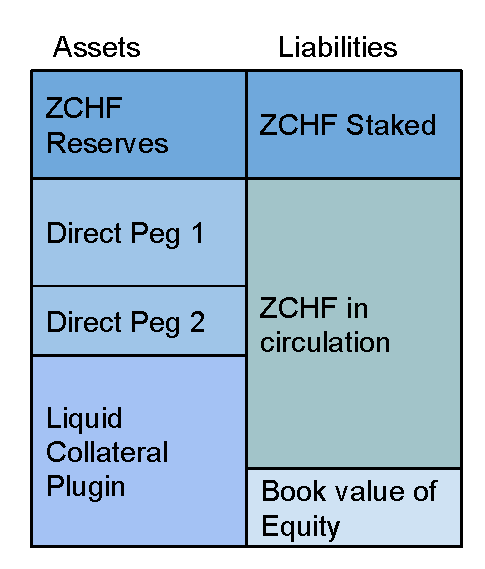
\includegraphics[width=0.25\textwidth]{FCBalanceSheet.pdf}
    \caption{\textbf{Balance Sheet}. This diagram
    schematizes the balance sheet of the Frankencoin system for
    a specific mint plugin setup.}\label{fig:bs}
\end{figure}

We motivate the following risk mitigating measures from 
the Basel III banking regulation and the Dodd-Frank Act, see, e.g., \cite{basel3}
and \cite{acharya2010regulating}:
\begin{enumerate}
\item \emph{Risk-based capital requirements}: each mint-plugin defines its own
	risk-based reserve requirement. E.g., for the liquid collateral
	plugin, we choose to estimate a reserve requirement based on expected shortfall.
	The fact that the system used shared capital but individual reserve requirements
	adds a diversification benefit.
\item \emph{Leverage limits} provide a supplementary measure to
	risk-based capital requirements due to their simplicity and independency. 
	It is a safeguard against model risk and was introduced with the
	Basel III regulation. Our system is subject to model risk too, for instance
	due to the risk-based calibration of the Liquid Collateral Plugin capital
	reserve, and we thus define leverage limits too.
\item \emph{Countercyclical buffer}: risk-based capital requirements
	show cyclicality. In crisis times, more capital is required
	than during expansionary periods. It is more difficult to
	attract capital in exactly these times. Therefore we
	introduce a countercyclical buffer, that governance reduces
	in downturns and increases during expansionary periods.\footnote{E.g., 
	loss given default is typically higher
	in a crisis. The Basel II framework required banks to use downturn LGD
	estimates to dampen countercyclicality, see \cite{engelmann2006basel}.
	Basel III introduced a countercyclical buffer to dampen the cyclicality
	emphasized by the banking system}
\item \emph{Concentration limits}. If the collateral of Frankencoin
	is singularly exposed to the price of Bitcoin, the Frankencoin is doomed
	to collapse when the Bitcoin price falls sufficiently. We therefore aim
	to limit the concentration of collateral. 
\end{enumerate}

If the capital is below the minimal capital derived from the above measures,
no more Frankencoins can be issued.
The above measures provide us with a capital requirement per ZCHF issued.
We propose to define the \emph{countercyclical buffer} as a multiplicative add-on to the
capital requirement resulting from the remaining measures. That is,
if the requirement from 1, 2, and 4 result in a buffer of $C$, the
countercyclical buffer is a number $b$, so that the minimal capital is equal
to $C(1+b)$. The system-wide buffer $b$ is set by governance.

We have detailed the \emph{risk-based capital} requirements in the previous sections.
The risk-based capital requirements involve relatively complex calculations
(for current blockchain capabilities), however, they are done off-chain and we are only required to store the resulting
parameters in the blockchain.

A simple way to measure \emph{concentration} is the one-firm concentration ratio,
see \cite{curry1983industrial}, which equals the percentage of market share held by the largest firm. We apply this to our context. Let $K$ be the number of mint plugins. Each mint plugin tracks the amount of ZCHF issued and not burned, $Z_j$.\footnote{Direct Peg Plugins
do not have the notion of a position and therefore set $Z_j$ equal to the
collateral. If collateral is liquidated, the ZCHF burnt are subtracted from
$Z_j$.}
The relative amount issued by plugin $j$ is given by $p_j=Z_j/\sum_i^K Z_i$. We aim to prevent that the largest
$p_j$ is beyond a threshold $\theta_C$. If a single mint plugin reaches the threshold 
$\theta_C$,
the plugin cannot issue any more ZCHF until the concentration is reduced. The
concentration threshold is set by governance.

Finally, we detail the \emph{leverage limits}. In the spirit of the
creators of the leverage limits, we aim to have the least possible assumptions
to define leverage limits in our system. We therefore do not want to rely on any 
collateral valuations or distributional assumptions.
Direct Peg Plugins should not count towards the leverage ratio,
because their value is stable and diversified through the concentration limits,
and because they provide a convenient way to issue new 
ZCHF that are subsequently staked. However, we want to limit the
amount of ZCHF issued through Liquid Collateral Plugins relative to the ZCHF
held as a reserve in the staking pool. We therefore define the leverage ratio
as
\begin{align}
LR = \sum_{i \in \mathcal{C}} Z_i/S,
\end{align}
where $Z_i$ is the amount of tokens issued by mint plugin $i$, $\mathcal{C}$
is the set of plugin indices that are to be included in the leverage
calculation (i.e., not the Direct Peg plugins), and $S$ is the total amount
of staked ZCHF. If the leverage ratio is larger than a governance set threshold $\theta_L$,
plugins other than the Direct Peg plugins can no longer mint ZCHF.

\begin{table}[htbp]
 \caption{\textbf{Summary of Data used in Smart Contracts.}
    This table lists the parameters and data that needs to
    be stored to implement the desired risk mitigation measures.} % title of Table
    \centering % used for centering table
\begin{tabularx}{\textwidth}{llX}
\toprule
Element To Store & Type & Description \\
\midrule
$Z_i$                        & Data          & Each mint plugin keeps track of ZCHF issued by the plugin and not burned                                     \\
$Z$, $Z^{\mathcal{C}}$ & Data          & The governance contract keeps track of the sum of $Z_i$ and the sum over the $Z_i$ issued by leverage constraint relevant contracts\\
$S$                         & Data          & Amount of ZCHF staked                                                                                        \\
$\mathcal{C}=\{c_0, ...,c_{N-1}\} \in \{0,1\}^N$               & Parameter     & Each mint plugin defines whether they are part of the leverage ratio calculation or not                      \\
$h$, $\tau$, $k$                 & Parameter     & Parameters for Liquid Collateral Plugin                                                                    \\
$\Theta^{(L)}$                   & Parameter     & Maximal leverage ratio                                                                                       \\
$\Theta_i^{(C)}$             & Parameter     & Maximal relative amount of ZCHF issued by mint plugin $i$ to limit concentration risk                                                  \\
$\Theta_i^{(F)}$             & Parameter     & Each mint plugin has a minting fee                                                                           \\
$\Theta_i^{(R)}$             & Parameter     & Each mint plugin sets its own risk-based reserve requirement, relative to the issued ZCHF                     \\
$\Theta_i^{(I)}$                        & Parameter     & Each mint plugin can define an interest rate paid to stakers (can be zero, e.g., in case of Direct Peg Plugins)\\
\bottomrule
\end{tabularx}\label{tab:summary}
\end{table}

Table~\ref{tab:summary} summarizes the parameters and data that needs to be
stored to implement these risk measures. Despite the comprehensive
measures, there are only a few parameters that need to be stored.

\emph{TODO: address how credit issuance works. Proposal: last price * 1.8 loan amount}
\clearpage
\section{Conclusion}
TODO

\newpage
\bibliographystyle{apalike}
\bibliography{references}

\clearpage
\appendix
\section{Data}\label{appx:data}
\begin{figure}[h]
    \center
    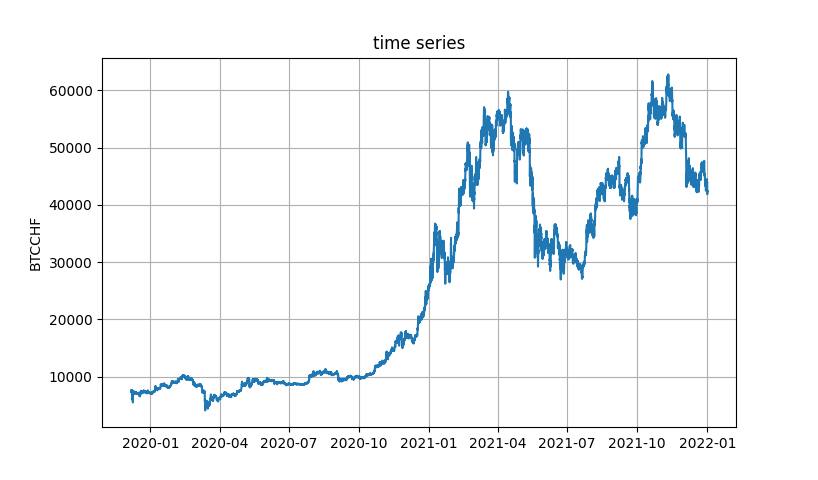
\includegraphics[width=0.75\textwidth]{time_series.png}
    \caption{\textbf{BTCCHF Level Data}. This figure plots
    the level data of the BTCCHF time-series. 
    We have 756 observations of daily candle data without gaps from 2019-12-07 to
    2021-12-31.}\label{fig:timeseries}
\end{figure}

We gather 1-hour candle data from Kraken, consisting of a timestamp, open, low,
high, close, number of trades, and volume.\footnote{See \url{https://support.kraken.com/hc/en-us/articles/360047124832-Downloadable-historical-OHLCVT-Open-} \url{High-Low-Close-Volume-Trades-data}}
From each open and close price we calculate 24h log-returns. Our return data has the following summary statistics.
\begin{table}[!h]
\caption{\textbf{Summary Statistics for 24h log-return data}.}
%\begin{center}
\centering
\begin{tabular}{lr}
\hline
num. observations & 756\\
min, max &[-49.09\%, 25.13\%] \\
mean & 0.26\% \\
variance & 0.0019 \\ 
skewness & -2.07 \\
kurtosis & 27.31 \\
\hline
\end{tabular}
%\end{center}
\end{table}
Table~\ref{tab:adf} test the time-series of 24h log-returns for stationarity via Augmented Dickey-Fuller test and rejects the null-hypothesis
of non-stationarity.
\begin{table}[!h]
\caption{\textbf{Stationarity Test}. The ADF test suggests that the log-return data is stationary.\label{tab:adf}}
\centering
\begin{tabular}{lrr}
\hline
ADF Statistic: &-12.6\\
p-value: &0.000000\\
Critical Value for 1\%:& -3.4\\
\hline
\end{tabular}
\end{table}

Figure~\ref{fig:qqplots} present a quantile-quantile plot against the normal distribution
and a histogram.


\begin{figure}[h]
    \center
    \begin{tabular}{ll}
    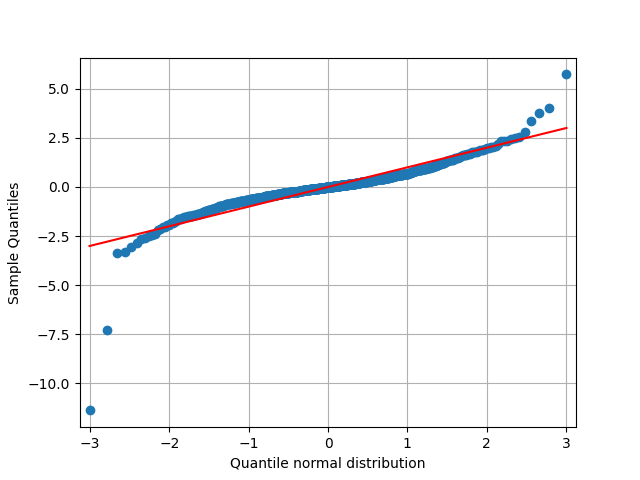
\includegraphics[width=0.5\textwidth]{qq_normal_kraken24h.png} &
    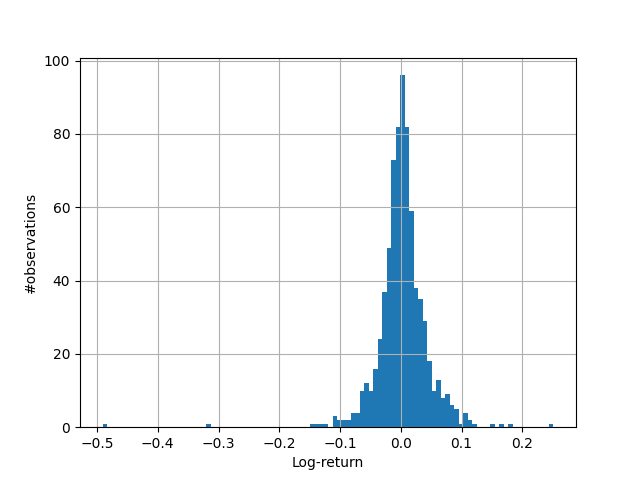
\includegraphics[width=0.5\textwidth]{hist24hreturns_kraken.png} \\
    \end{tabular}
    \caption{\textbf{Return Data from Kraken}. The lhs plot shows a quantile-quantile plot
    of the 24h log-return data against a normal distribution, the rhs
    plots a histogram of the 24h log-returns.
    From the lhs graph we see that we have more extreme returns than what a normal
    distribution would suggest. In the center of the distribution, the 
    returns move less than the normal distribution would imply.}\label{fig:qqplots}
\end{figure}


\end{document}